\documentclass[usenames,dvipsnames,10pt,aspectratio=169]{beamer} 
% Add option 'aspectratio=169' for 16:9 widescreen 
% Add option  'handout' to ignore animations
% If you have a smaller amount of text, feel free to also try '11pt'! / Jesper

\usepackage[utf8]{inputenc}
\usepackage{verbatim}
\usepackage{minted}
\usemintedstyle{monokai}
\usepackage{graphicx}
\usepackage{wrapfig}
\usepackage[document]{ragged2e}
\usetheme{umu}

\usepackage{hyperref}
\hypersetup{
    colorlinks=true,
    linkcolor=ucuyellow,
    filecolor=ucuyellow,      
    urlcolor=ucuyellow,
}
\urlstyle{same}

%%% Bibliography
\usepackage[style=authoryear,backend=biber]{biblatex}
\addbibresource{bibliography.bib}

\DeclareNameAlias{author}{given-family}

%%% Suppress biblatex annoying warning
\usepackage{silence}
\WarningFilter{biblatex}{Patching footnotes failed}

%%% Some useful commands
% pdf-friendly newline in links
\newcommand{\pdfnewline}{\texorpdfstring{\newline}{ }} 
% Fill the vertical space in a slide (to put text at the bottom)
\newcommand{\framefill}{\vskip0pt plus 1filll}

%%% Enter additional packages below (or above, I can't stop you)! / Jesper
\renewcommand{\proofname}{\sffamily{Proof}}

%%%%%%%%%%%%%%%%%%%%%%%%%%%%%%%%%%%%%%%%%%%%%%%%%%%%%%%%%%%%%%%%%%%%%%%%%%%%%%%%%%%%%
\title[Rust \#1]{Rust \#1: Motivation and Introduction}
\date[\today]{\small\today}
\author[Sultanov Andriy]{Sultanov Andriy}
\institute{APPS@UCU}

\begin{document}

\begin{frame}
\titlepage
\end{frame}

\begin{frame}{\contentsname}
\tableofcontents
\end{frame}

\framepic{graphics/1.jpg}{
 \textcolor{ucuwhite}{A short history of systems programming}
 \vskip 0.5cm
 }

\section{A short history of systems programming}
\begin{frame}{The origins of C}

\begin{wrapfigure}{r}{0.5\textwidth}
\centering
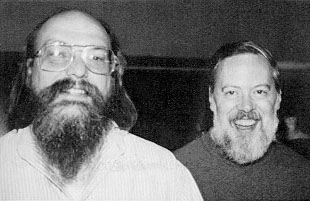
\includegraphics[width=0.5\textwidth]{graphics/ritchie.jpg}
\end{wrapfigure}
\normalsize
The C programming language appeared during Unix development in 1972.\\

Since it was created for a specific purpose % an operating system
and a specific computer, %(PDP-11) 
on the one hand it adapted to the
needs of the programmers, and on the 
other it adopted a large
amount of somewhat unique and unpopular 
ideas and concepts.

\vskip 0.8cm

\end{frame}

\begin{frame}{Possible solutions}
\large
C++ is born to help address some of these problems,\\ 
introduces ‘zero cost’ abstractions, aimed at providing\\
a nice interface for the programmer to use which\\
compiles down to an almost ideal machine code.
\vspace{0.5cm}

Still has the old instruments, hangs on to C's machine\\
model %(the fucking BACKWARDS COMPATIBILITY),
and tries to encourage using the new\\ 
modern safe concepts, 
\href{https://alexgaynor.net/2019/apr/21/modern-c++-wont-save-us/}
{which are not ideal either}.


\end{frame}

\begin{frame}{Modern ideas}

\large
In the meantime, languages like Java, Ruby and\\
Python start sprawling up, presenting another\\
model of growth - they are garbage-collected\\
and are able to present even more complex\\
abstractions (at the expense of the speed).\\

\vspace{0.5cm}

Go and others try to tackle C's speed and\\
low-levelness, 
\href{https://cowlark.com/2009-11-15-go/}{unsuccessfully}.

\end{frame}

\framepic{graphics/1.jpg}{
 \textcolor{ucuwhite}{Pitfalls of the old ways}
 \vskip 0.5cm
 }

\section{Pitfalls of the old ways}

\begin{frame}{General stuff} 
	General stuff about how they are not memory-safe.
	

	*Should probably spend some time explaining the memory layout,
	so it'd be possible to explain buffer overflows, dangling 
	pointers and null pointers.*
\end{frame}

\begin{frame}{Buffer overflows} 
	\inputminted[fontsize=\large]{c}{code/overflow.c}
\end{frame}

\begin{frame}{Null pointers}
	\inputminted[fontsize=\large]{c}{code/nullp.c}
\end{frame}

\begin{frame}{Dangling pointers} 
	\inputminted[fontsize=\large]{c}{code/danp.c}
\end{frame}

\begin{frame}{Invalidated iterators} 
	\inputminted[fontsize=\large]{c}{code/iter.c}
\end{frame}

\begin{frame}{No real error checking} 
	\inputminted[fontsize=\large]{c}{code/errorcheck.c}
\end{frame}

\begin{frame}{And many more...}
	\large
	\begin{itemize}
		\item Memory leak - you can forget to free data
		\item Thread unsafety - another function can be modifying the same memory
		\item Double free - you can free the same memory twice (as a part of a struct, for example)
	\end{itemize}
\end{frame}


\framepic{graphics/1.jpg}{
 \textcolor{ucuwhite}{Where and why is Rust better?}
 \vskip 0.5cm
 }

\section{Where and why is Rust better?}

\begin{frame}{What is Rust?}

	\LARGE{\textcolor{ucuyellow}{Safe, Fast, Easy to write. Choose three}}

\vspace{0.8cm}
\large
A modern system programming language.

\vspace{0.3cm}

First stable version in 2014.\\
Gets rid of unnecessary old ideas, \\
combining them with some of the\\
fresh concepts.
\end{frame}

\begin{frame}{Almost everything makes sense} 

\large
It does not care about C’s old ways\\ 
from the 70s which have been kept up \\
in many languages and systems since.\\ 
%just because (null-char strings, pointers) 

\vspace{0.3cm}
It does not try to needlessly attach new\\ 
stupid things to it. Easily gets rid of bad\\ 
ideas since it’s a young language.\\
\end{frame}

\begin{frame}{Memory safety guarantees}
\large
Rust guarantees, at compile time, that\\
programs are memory-safe.\\

\vspace{0.3cm}

This means:
\begin{itemize}
	\item No buffer overflows
	\item Everything is bounds-checked\\ (e.g. no null pointers, no dangling pointers)
	\item No data races (general thread-safety)
	\item No memory is ever written to by two things at a time
	\item No memory is ever written and read at the same time
\end{itemize}
\end{frame}

\begin{frame}{Tradeoffs}
\large
These guarantees don't\\
come without a cost.

\vspace{0.3cm}

Some of them include:
\begin{itemize}
	\item Relatively long compile time
	\item You sometimes have to fight with the compiler\\
		(It's always right though, and even tries to help)
	\item A whole new different approach to things
	\item It's a young language!\\
		(This also means you can help)
\end{itemize}
\end{frame}

\begin{frame}{Improvements in almost every field} 
	\large
Rust does not only get rid of the problems\\
of C and garbage-collected languages.
\vspace{0.3cm}

It tries to be better at a lot of other things:
\begin{itemize}
	\item Super great error handling!
	\item Algebraic data types!\\
		(Functional programming concept)
	\item Advanced macro processing!
	\item Speed increase from C since programs \\
		often know what to expect!
\end{itemize}
\end{frame}

\begin{frame}{An amazing ecosystem} 
Modern languages are not only language\\
specifications. Their use almost always\\
depends on compilers, package management\\
systems, documentation, formatters, and\\
test suites!
\vspace{0.25cm}

\large
And Rust has a great ecosystem:
\begin{itemize}
	\item rustc compiler is super helpful, and has great IDE integrations!
	\item cargo is a unified standard for:
		\begin{itemize}
			\item Package management (pip, yay)
			\item Dependency resolving (setup.py, requirements.txt)
			\item Project management (makefile, CMake)
			\item Testing (gtest etc.)
			\item Documentation (pandoc, asciidoc etc.)
		\end{itemize}
	\item rustfmt is a standard formatter
\end{itemize}
\end{frame}

\framepic{graphics/1.jpg}{
 \textcolor{ucuwhite}{Basic syntax and concepts}
 \vskip 0.5cm
 }

\section{Basic syntax and concepts}

\begin{frame}{Hello world!}

	\inputminted[fontsize=\Large]{c}{code/helloworld.rs}

\end{frame}

\begin{frame}{Hello cargo!}

	\inputminted[fontsize=\Large]{c}{code/hellocargo.rs}

\end{frame}

\framepic{graphics/1.jpg}{
	\textcolor{ucuwhite}{The Rust ecosystem\\ and a little more...}
 \vskip 0.5cm
 }

\section{The Rust ecosystem and a little more}

\begin{frame}{Guessing game}
	\framesubtitle{Basics}
	*Type system explanation, print macros, expect() and methods*
	\inputminted[fontsize=\normalsize]{c}{code/guess1.rs}
\end{frame}

\begin{frame}{Guessing game}
	\framesubtitle{Cargo dependencies}
	\Large
	*Explain how dependencies work.\\
	Or at least try to.*
	\vspace{0.5cm}

	Add this to your Cargo.toml file:
	\inputminted[fontsize=\Large]{c}{code/toml1.toml}
\end{frame}

\begin{frame}{Guessing game}
	\framesubtitle{Random number generation}
	\inputminted[fontsize=\footnotesize]{c}{code/guess2.rs}
\end{frame}

\begin{frame}{Guessing game}
	\framesubtitle{(Wrong) Input comparison}
	*Match expression, enumerators explanation.*
	\inputminted[fontsize=\normalsize]{c}{code/guess3.rs}
\end{frame}

\begin{frame}{Guessing game}
	\framesubtitle{Input comparison}
	*Ownership explanation, maybe add a slide about that?*
	\inputminted[fontsize=\normalsize]{c}{code/guess4.rs}
\end{frame}

\begin{frame}{Ownership and lifetimes}
	\framesubtitle{General}
	\normalsize
	Rust enforces its own (rational) system of ownership\\
	and lifetimes. A few main points:
	\begin{itemize}
		\item Borrowing
		\begin{itemize}
			\item We can have multiple shared (immutable) references\\
				at once (with no mutable references) to a value.
			\item We can have only one mutable reference\\
				at once (no shared references to it)
		\end{itemize}
		\item Lifetimes
		\begin{itemize}
			\item The lifetime of a value starts when it’s created\\
				and ends the last time it’s used
			\item Rust doesn’t let you have a reference to a value\\
				that lasts longer than the value’s lifetime
			\item Rust computes lifetimes at compile time,\\
				there are no allocations and frees,\\
				Rust only borrows and drops memory
		\end{itemize}
	\end{itemize}
\end{frame}

\begin{frame}{Ownership and lifetimes}
	\framesubtitle{Examples}
	\inputminted[fontsize=\normalsize]{c}{code/own1.rs}
	\vspace{0.6cm}
	\inputminted[fontsize=\normalsize]{c}{code/own2.rs}
\end{frame}

\begin{frame}{Ownership and lifetimes}
	\framesubtitle{Examples}
	\inputminted[fontsize=\large]{c}{code/own3.rs}
\end{frame}

\begin{frame}{Guessing game}
	\framesubtitle{Looping}
	\inputminted[fontsize=\normalsize]{c}{code/guess5.rs}
\end{frame}

\begin{frame}{Guessing game}
	\framesubtitle{Breaking out of the loop}
	\inputminted[fontsize=\normalsize]{c}{code/guess6.rs}
\end{frame}

\begin{frame}{Guessing game}
	\framesubtitle{Handling invalid input}
	\inputminted[fontsize=\normalsize]{c}{code/guess7.rs}
\end{frame}

\begin{frame}{More on cargo}
	\inputminted[fontsize=\normalsize]{shell}{code/cargo.sh}
\end{frame}

\framepic{graphics/1.jpg}{
	\textcolor{ucuwhite}{Thank you!}
 \vskip 0.5cm
 }

\begin{frame}{Interesting readings} 
\href{https://web.archive.org/web/19980425023657/http://paul.merton.ox.ac.uk/computing/unix.html}
{Creators Admit UNIX, C Hoax}

\href{https://web.archive.org/web/19990302094922/http://www.elj.com/cppcv3/}
{C++?? : A Critique of C++ (or Programming and Language Trends of the 1990s)}

\href{https://web.archive.org/web/20030625015044/http://www.cs.rice.edu/CS/PLT/Teaching/Talks/TCEA-State-1998/C++/}
{Mastering the AP CS Curriculum Without Using C++}

\href{https://matklad.github.io/2020/09/20/why-not-rust.html}
{Why not Rust?}

\href{https://matklad.github.io/2020/02/14/why-rust-is-loved.html}
{Why is Rust the Most Loved Programming Language?}

\href{https://da-data.blogspot.com/2020/10/no-c-still-isnt-cutting-it.html}
{No, C++ still isn't cutting it.}

\href{http://dtrace.org/blogs/bmc/2018/09/18/falling-in-love-with-rust/}
{Falling in love with Rust}

\href{http://dtrace.org/blogs/bmc/2020/10/11/rust-after-the-honeymoon/}
{Rust after the honeymoon}

\href{http://dtrace.org/blogs/bmc/2018/09/28/the-relative-performance-of-c-and-rust/}
{The relative performance of C and Rust}

\end{frame}

\end{document}
